\documentclass[
	% -- opções da classe memoir --
	12pt,					% tamanho da fonte
	openright,				% capítulos começam em pág ímpar (insere página vazia caso preciso)
	oneside,					% para impressão em verso e anverso. Oposto a twoside
	a4paper,					% tamanho do papel. 
	% -- opções da classe abntex2 --
	%chapter=TITLE,			% títulos de capítulos convertidos em letras maiúsculas
	%section=TITLE,			% títulos de seções convertidos em letras maiúsculas
	%subsection=TITLE,		% títulos de subseções convertidos em letras maiúsculas
	%subsubsection=TITLE,	% títulos de subsubseções convertidos em letras maiúsculas
	% -- opções do pacote babel --
	english,					% idioma adicional para hifenização
	%french,					% idioma adicional para hifenização
	%spanish,				% idioma adicional para hifenização
	brazil					% o último idioma é o principal do documento
	]{abntex2}

% ---------------------
% Pacotes OBRIGATÓRIOS
% ---------------------
\usepackage{lmodern}				% Usa a fonte Latin Modern			
\usepackage[T1]{fontenc}			% Selecao de codigos de fonte.
\usepackage[utf8]{inputenc}		% Codificacao do documento (conversão automática dos acentos)
\usepackage{lastpage}			% Usado pela Ficha catalográfica
\usepackage{indentfirst}		% Indenta o primeiro parágrafo de cada seção.
\usepackage{color}				% Controle das cores
\usepackage{graphicx,graphicx}	% Inclusão de gráficos
\usepackage{epsfig,subfig}		% Inclusão de figuras
\captionsetup[figure]{labelfont={bf},name={Fig.},labelsep=period}
\usepackage{microtype} 			% Melhorias de justificação
% ---------------------
		
% ---------------------
% Pacotes ADICIONAIS
% ---------------------
\usepackage{lipsum}						% Geração de dummy text
\usepackage{amsmath,amssymb,mathrsfs}	% Comandos matemáticos avançados 
\usepackage{setspace}  					% Para permitir espaçamento simples, 1 1/2 e duplo
\usepackage{verbatim}					% Para poder usar o ambiente "comment"
\usepackage{tabularx} 					% Para poder ter tabelas com colunas de largura auto-ajustável
\usepackage{afterpage} 					% Para executar um comando depois do fim da página corrente
\usepackage{url} 						% Para formatar URLs (endereços da Web)
% ---------------------

% ---------------------
% Pacotes de CITAÇÕES
% ---------------------
%\usepackage[brazilian,hyperpageref]{backref}	% Paginas com as citações na bibl
\usepackage[numbers,sort&compress]{natbib} 
%\usepackage[num]{abntex2cite}				% Citações padrão ABNT 
%\usepackage[alf]{abntex2cite}				% Citações padrão ABNT(autor-data)

%Tipo de simbolo
%\citebrackets[] 							 
%\citebrackets()
%\citebrackets{}

% ---------------------

% Configurações de CITAÇÕES para abntex2
%% --- 
% CONFIGURAÇÕES DE PACOTES
% --- 

% ---
% Configurações do pacote backref
% Usado sem a opção hyperpageref de backref
\renewcommand{\backrefpagesname}{Citado na(s) página(s):~}
% Texto padrão antes do número das páginas
\renewcommand{\backref}{}
% Define os textos da citação
\renewcommand*{\backrefalt}[4]{
	\ifcase #1 %
		Nenhuma citação no texto.%
	\or
		Citado na página #2.%
	\else
		Citado #1 vezes nas páginas #2.%
	\fi}%
% ---

% Inclusão de dados para CAPA e FOLHA DE ROSTO (título, autor, orientador, etc.)
\include{pretextual/ContraCapa}

% Inclui Configurações de aparência do PDF Final
%  Configurações de aparência do PDF final
% NÃO ALTERAR!!!

% alterando o aspecto da cor azul
\definecolor{blue}{RGB}{41,5,195}

% informações do PDF
\makeatletter
\hypersetup{
     	%pagebackref=true,
		pdftitle={\@title}, 
		pdfauthor={\@author},
    	pdfsubject={\imprimirpreambulo},
	    pdfcreator={LaTeX with abnTeX2},
		pdfkeywords={abnt}{latex}{abntex}{abntex2}{trabalho acadêmico}, 
		colorlinks=true,       		% false: boxed links; true: colored links
    	linkcolor=blue,          	% color of internal links
    	citecolor=blue,        		% color of links to bibliography
    	filecolor=magenta,      		% color of file links
		urlcolor=blue,
		bookmarksdepth=4
} 
\makeatother
% --- 

% O tamanho da identação do parágrafo é dado por:
\setlength{\parindent}{1.3cm}

% Controle do espaçamento entre um parágrafo e outro:
\setlength{\parskip}{0.2cm}  % tente também \onelineskip

% ---------------------
% Compila o indice
% ---------------------
\makeindex
% ---------------------

%%%%%%%%%%%%%%%%%%%%%%%%%%%
%%  INICIO DO DOCUMENTO  %%
%%%%%%%%%%%%%%%%%%%%%%%%%%%
\begin{document}

% Retira espaço extra obsoleto entre as frases.
\frenchspacing

% ----------------------------------------------------------
% ELEMENTOS PRÉ-TEXTUAIS (Capa, Resumo, Abstract, etc.)
% ----------------------------------------------------------
\pretextual

% Capa
% ---
% Impressão da Capa
% ---
\begin{capa}%
    \begin{center}
    	\begin{figure}[!htb]
    		%Logo GCOM
            
\includegraphics[scale=0.07]{imagens/unipac.jpg} 
    		\hfill
        		\begin{minipage}{10cm} \vskip -3cm
        		\ABNTEXchapterfont\large\center{Fundação Presidente Antônio Carlos\\ Conselheiro Lafaiete \\ Engenharia de Computação}
                \end{minipage}
    		% Logo da engenharia
    		
\includegraphics[scale=0.85]{imagens/eng.jpg}
    	\end{figure}
    \end{center}
    \center
	%\vspace{1.5cm}

    \vfill
    \ABNTEXchapterfont\bfseries\LARGE\imprimirtitulo
    \vfill

	%\vfill
	\ABNTEXchapterfont\large\imprimirautor
	\vfill
%
    \large\imprimirlocal, \large\imprimirdata

    \vspace*{1cm}
 \end{capa}
% ---

% Folha de rosto (o * indica que haverá a ficha bibliográfica)
\imprimirfolhaderosto*

% Imprimir Ficha Catalografica
%% ---
% Ficha Catalográfica
% ---
% Isto é um exemplo de Ficha Catalográfica, ou ``Dados internacionais de
% catalogação-na-publicação''. Você pode utilizar este modelo como referência. 
% Porém, provavelmente a biblioteca da sua universidade lhe fornecerá um PDF
% com a ficha catalográfica definitiva após a defesa do trabalho. Quando estiver
% com o documento, salve-o como PDF no diretório do seu projeto e substitua todo
% o conteúdo de implementação deste arquivo pelo comando abaixo:
%
% \begin{fichacatalografica}
%     \includepdf{fig_ficha_catalografica.pdf}
% \end{fichacatalografica}
\begin{fichacatalografica}
	\vspace*{\fill}					% Posição vertical
	\hrule							% Linha horizontal
	\begin{center}					% Minipage Centralizado
	\begin{minipage}[c]{12.5cm}		% Largura
	
	\imprimirautor
	
	\hspace{0.5cm} \imprimirtitulo  / \imprimirautor. --
	\imprimirlocal, \imprimirdata-
	
	\hspace{0.5cm} \pageref{LastPage} p. : il. (algumas color.) ; 30 cm.\\
	
	\hspace{0.5cm} \imprimirorientadorRotulo~\imprimirorientador\\
	
	\hspace{0.5cm}
	\parbox[t]{\textwidth}{\imprimirtipotrabalho~--~\imprimirinstituicao,
	\imprimirdata.}\\
	
	\hspace{0.5cm}
		1. Palavra-chave1.
		2. Palavra-chave2.
		I. Orientador.
		II. Universidade xxx.
		III. Faculdade de xxx.
		IV. Título\\ 			
	
	\hspace{8.75cm} CDU 02:141:005.7\\
	
	\end{minipage}
	\end{center}
	\hrule
\end{fichacatalografica}
% ---

% Inserir Folha de Aprovação
%% ---
% Assinaturas
% ---
% Isto é um exemplo de Folha de aprovação, elemento obrigatório da NBR
% 14724/2011 (seção 4.2.1.3). Você pode utilizar este modelo até a aprovação
% do trabalho. Após isso, substitua todo o conteúdo deste arquivo por uma
% imagem da página assinada pela banca com o comando abaixo:
%
% \includepdf{folhadeaprovacao_final.pdf}
%
\begin{folhadeaprovacao}

  \begin{center}
    {\ABNTEXchapterfont\large\imprimirautor}

    \vspace*{\fill}\vspace*{\fill}
    \begin{center}
      \ABNTEXchapterfont\bfseries\Large\imprimirtitulo
    \end{center}
    \vspace*{\fill}
    
    \hspace{.45\textwidth}
    \begin{minipage}{.5\textwidth}
        \imprimirpreambulo
    \end{minipage}%
    \vspace*{\fill}
   \end{center}
        
   Trabalho aprovado. \imprimirlocal, XX de XXXX de 202X:

   \assinatura{\textbf{\imprimirorientador} \\ Orientador} 
   \assinatura{\textbf{\imprimircoorientador} \\ Co-Orientador} 
   \assinatura{\textbf{Professor} \\ Convidado 1}
   \assinatura{\textbf{Professor} \\ Convidado 2}
   \assinatura{\textbf{Professor} \\ Convidado 3}
      
   \begin{center}
    \vspace*{0.5cm}
    {\large\imprimirlocal}
    \par
    {\large\imprimirdata}
    \vspace*{1cm}
  \end{center}
  
\end{folhadeaprovacao}
% ---

% Dedicatória
%% ---
% Dedicatória
% ---
\begin{dedicatoria}
   \vspace*{\fill}
   \centering
   \noindent
   \textit{ Aos meus pais XXXXXXXX e YYYYYYY, \\ por sempre estarem comigo em todos os momentos.} \vspace*{\fill}
\end{dedicatoria}
% ---

% Agradecimentos
% ---
% Agradecimentos
% ---
\begin{agradecimentos}

Agradeço a Deus por me iluminar nos momentos difíceis, dando força na longa caminhada.

Em especial minha esposa, por me apoiar incondicionalmente e por sempre confiar em meu potencial me incentivando a fazer sempre o melhor e a meu filho pelas risadas calorosas que me renovam sempre o ânimo e me lembram dos meus objetivos.

%Aos meus irmãos, por.....

Ao meu orientador Alex Vitorino por sua paciência e sempre propondo novos desafios que são de grande contribuição em relação ao meu aprendizado e com ensinamentos importantes para consolidação deste trabalho.

%Aos meus amigos ...

%Aos professores ...

%À XXXXXX pelo apoio financeiro para realização deste trabalho de pesquisa.

Enfim em todos que acreditaram no meu sonho.

\end{agradecimentos}
%% ---

% Epígrafe
% ---
% Epígrafe
% ---
\begin{epigrafe}
    \vspace*{\fill}
	\begin{flushright}
		\textit{``A mão queimada ensina melhor. \\
		          Depois disso o conselho sobre o fogo \\
                  chega ao coração.''-- Gandalf - O Cinzento \\
		          (J.R.R. Tolkien)}
	\end{flushright}
\end{epigrafe}
% ---

% Resumo e Abstract
% ---
% RESUMOS
% ---

% RESUMO em português
\setlength{\absparsep}{18pt} % ajusta o espaçamento dos parágrafos do resumo
\begin{resumo}
    O objetivo deste presente trabalho é a consolidação dos conhecimentos adquiridos durante a realização da disciplina de Sistemas Operacionais, dando enfoque aos sistemas baseados em Linux utilizados em servidores, salientando suas utilizações e o seu mercado de atuação. \\
    O Linux é um sistema operacional que vive em um crescimento contínuo e é amplamente usado ele está tanto em sensores a supercomputadores, e podemos vê-lo sendo usados em espaçonaves, automóveis, \emph{smartphones}, relógios e muitos outros dispositivos em nossa vida cotidiana \cite{LinuxFundationWIL}.\\
    Em especial o sistema Linux é um sistema de código aberto o que significa que é possível executá-lo para qualquer propósito, estudar seu funcionamento e modificá-lo se assim desejar, ou realizar cópias para terceiros dando total liberdade para sua comunidade \cite{LinuxFundationWIL},\cite{Morimoto2011}.\\
    Ele também opera a maior parte da Internet, todos os 500 maiores supercomputadores do mundo e as bolsas de valores do mundo. Estes funcionam em uma variação do Linux preparada para um grande fluxo de tratamento de dados, podendo rodar vários serviços simultaneamente, esta versão é a Linux para servidores ou \emph{Linux Server} \cite{LinuxFundationWIL},\cite{Morimoto2011}.\\





 \textbf{Palavras-chaves}: Linux, Servidores, Sistema Operacional.
\end{resumo}

% ABSTRACT in english
% \begin{resumo}[Abstract]
%  \begin{otherlanguage*}{english}
%   This is the english abstract.

%   \vspace{\onelineskip}
 
%   \noindent 
%   \textbf{Keywords}: latex. abntex. text editoration.
%  \end{otherlanguage*}
% \end{resumo}

% Lista de ilustrações
\pdfbookmark[0]{\listfigurename}{lof}
\listoffigures*
\cleardoublepage

% Lista de tabelas
\pdfbookmark[0]{\listtablename}{lot}
\listoftables*
\cleardoublepage

% Lista de abreviaturas e siglas
\begin{siglas}
    \item[E/S] Entrada e saída
    \item[FreeBSD] Free OS descended from the 
    Berkeley Software Distribution 
    \item[GNU] GNU's Not Unix
    \item[GNU GPL] GNU General Public License
    \item[GUI] Graphical User Interface
    \item[MIT] Massachusetts Institute of Technology
    \item[MULTICS] MULTiplexed Information and Computing Service 
    \item[OS] Operating System  
    \item[OS X] Operating Systems number 10 
    \item[PC] Personal Computer
    \item[SO] Sistema Operacional
\end{siglas}

% Lista de símbolos
%\begin{simbolos}
  \item[$ \Gamma $] Letra grega Gama
  \item[$ \Lambda $] Lambda
  \item[$ \zeta $] Letra grega minúscula zeta
  \item[$ \in $] Pertence
\end{simbolos}

% Inserir o SUMÁRIO
\pdfbookmark[0]{\contentsname}{toc}
\tableofcontents*
\cleardoublepage

% ----------------------------------------------------------
% ELEMENTOS TEXTUAIS (Capítulos)
% ----------------------------------------------------------
\textual
% Elementos textuais com numeração arábica
\pagenumbering{arabic}
% Reinicia a contagem do número de páginas
\setcounter{page}{1}

% Inclui cada capitulo da Dissertação
% ----------------------------------------------------------
% Introdução 
% Capítulo sem numeração, mas presente no Sumário
% ----------------------------------------------------------

\chapter[Introdução]{Introdução}
%\addcontentsline{toc}{chapter}{Introdução}

Um computador moderno consiste em um emaranhado de peças que contém um ou mais processadores, alguma memória principal, alguma memória secundaria, interfaces de rede diversos periféricos como impressoras, teclado, mouse, monitor e vários outros dispositivos de entrada e saída. Podemos dizer que este é um sistema complexo, para realizar a desafiadora maratona que é compreender como cada parte funciona e gerenciar com maestria esses componentes é um grande desafio \cite{Tanenbaum2016}.\\
Para isso os computadores modernos são equipados com um SO esse dispositivo de \emph{software} tem a função de fornecer uma plataforma simples e limpa para o usuário de forma a ajuda-lo nas entradas e saídas de dados. Em uma visão simplista podemos ver na figura \ref{fig:figura1} onde o SO se encontra em relação entre \emph{hardware} e o usuário \cite{Tanenbaum2016}. 

\begin{figure}[htpb]
    \centering
   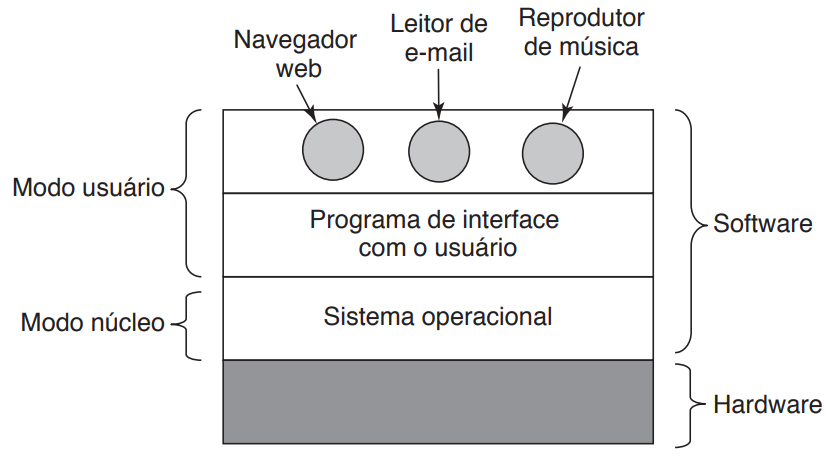
\includegraphics[scale=.4]{imagens/figura1.png}
   \caption{Onde o sistema operacional se encaixa. \cite{Tanenbaum2016}}
   \label{fig:figura1}
\end{figure}

Inicialmente a ideia que temos de um SO é a visão que temos dos ditos sistemas operativos que temos conhecimento que podem ser \emph{Windows}, \emph{Linux}, \emph{FreeBSD}, ou \emph{OS X} mas normalmente a forma de interagir com diretamente com o sistema é através de terminais comumente conhecidos como shell (interpretadores de comando) isto quando baseado em texto ou \emph{GUI (Graphical User Interface)} quando em modo gráfico \cite{Tanenbaum2016}.\\
Um sistema operacional é projetado para ocultar as particularidades de \emph{hardware} (ditas "de baixo nível") e assim criar uma máquina abstrata que fornece às aplicações serviços compreensíveis ao usuário (ditas "de alto nível") \cite{Comer2012}.\\
Assim o sistema trabalha em dois estados o modo núcleo e o modo usuário. Sendo que no modo núcleo (também chamado modo supervisor ou \emph{Kernel mode}). O sistema tem acesso completo aos recursos seja de ao \emph{hardware} ou \emph{software} e pode executar qualquer instrução que a máquina for capaz de executar \cite{Tanenbaum2016}, \cite{linfo2007}.\\
Quando o sistema está em modo \emph{kernel} é considerado que as execuções são de uma fonte confiável e, portanto, pode executar quaisquer instruções e fazer referência a quaisquer endereços de memória (ou seja, locais na memória). O \emph{kernel} tem total controle sobre o sistema e trata todos os outros \emph{software}s como programas não confiáveis, assim todas as operações em modo usuário que necessitem alterar o sistema solicitam ao uso do \emph{kernel} por meio de uma chamada de sistema  para executar instruções privilegiadas, como criação de processos ou operações de entrada / saída \cite{Tanenbaum2016}, \cite{linfo2007}.\\

Neste trabalho iremos trabalhar com o sistemas baseados em \emph{Linux} para servidores mas é importante entender um pouco da evolução desse sistema.

Em meados da década de 60 uma iniciativa conjunta do \emph{MIT}, da \emph{Bell Labs}  e da \emph{General Electric} decidiram embarcar no desenvolvimento de um “computador utilitário”, isto é, uma máquina que daria suporte a algumas centenas de usuários simultâneos em pouco tempo nasce o projeto MULTICS (Serviço de Computação e Informação Multiplexada) \cite{Tanenbaum2016}.\\
O MULTICS foi projetado para ser um sucesso com suporte para centenas de usuários em uma máquina apenas um pouco mais poderosa do que um PC baseado no 386 da \emph{Intel}. Mas transformá lo em um produto final de fácil comercialização não foi amarga realidade \cite{Tanenbaum2016}.\\
A \emph{Bell Labs} abandonou o projeto, e a \emph{General Electric} abandonou completamente o negócio dos computadores. Entretanto, o \emph{MIT} persistiu e finalmente colocou o MULTICS para funcionar.E foi instalado por mais ou menos 80 empresas e universidades importantes mundo afora \cite{Tanenbaum2016}.\\
Um dos cientistas da \emph{Bell Labs} que havia trabalhado no projeto MULTICS, Ken Thompson, decidiu escrever uma versão despojada e para um usuário do MULTICS. Esse trabalho mais tarde desenvolveu-se no sistema operacional UNIX, que se tornou popular no mundo acadêmico, em agências do governo e em muitas empresas \cite{Tanenbaum2016}.\\
Em 1987, Andrew Tanenbaum lançou um pequeno clone do UNIX, chamado MINIX, para fins educacionais. Em termos funcionais, o MINIX é muito similar ao UNIX \cite{Tanenbaum2016}.\\
Em 1991 Linus Torvalds começou um projeto inicialmente um emulador de terminal que era utilizado para acessar os servidores em UNIX da universidade Helsinki. Ele escreveu o código para especificamente  para o \emph{hardware} que utilizava um computador com um processador 80386 ele realizou o desenvolvimento no minix usando o \emph{GNU C compiler} \cite{Torvalds1991}, \cite{Torvalds1993}, \cite{torvalds2002}.\\
O \emph{Linux} também é distribuído sob uma licença de código aberto. O código aberto segue estes locatários principais:
\begin{itemize}
    \item A liberdade de executar o programa, para qualquer propósito.
    \item A liberdade de estudar como o programa funciona e alterá-lo para que ele faça o que você deseja.
    \item A liberdade de redistribuir cópias para que você possa ajudar seu vizinho.
    \item A liberdade de distribuir cópias de suas versões modificadas para terceiros.
\end{itemize}
Esses pontos são cruciais para entender a ideia por trás do \emph{Linux}. O \emph{Linux} se transformou em um sistema de fácil acesso. Com a grande liberdade de se poder modificar o sistema ele proporcionou a criação de diversas distribuições uma vez que qualquer usuário pode criar uma que atenda a suas necessidades \cite{LinuxFundationWIL}.\\
Nos próximos sessões  iremos discutir sobre o sistema e aprofundar no \emph{Linux} para assim entender, suas funcionalidade, modo de funcionamento e  quais suas principais atuações.\\









%\section*{Figuras}\label{sec:figuras}
%\addcontentsline{toc}{section}{figuras}

% \section*{Tabelas}\label{sec:tabelas}
% \addcontentsline{toc}{section}{tabelas}

%\section*{Motivação}\label{sec:motivacao}
%\addcontentsline{toc}{section}{Motivação}

%\section*{Objetivos}\label{sec:objetivos}
%\addcontentsline{toc}{section}{Objetivos}




% PARTE - Define a divisão do documento em partes (Não é obrigatório)
%\part{Preparação da pesquisa}
%% ---
\chapter{Uso de referências bibliográficas}
% ---

A formatação das referências bibliográficas conforme as regras da ABNT são um
dos principais objetivos do \abnTeX. Consulte os manuais
\citeonline{abntex2cite} e \citeonline{abntex2cite-alf} para obter informações
sobre como utilizar as referências bibliográficas.

%-
\subsection{Acentuação de referências bibliográficas}
%-

Normalmente não há problemas em usar caracteres acentuados em arquivos
bibliográficos (\texttt{*.bib}). Porém, como as regras da ABNT fazem uso quase
abusivo da conversão para letras maiúsculas, é preciso observar o modo como se
escreve os nomes dos autores. Na~\autoref{tabela-acentos} você encontra alguns
exemplos das conversões mais importantes. Preste atenção especial para `ç' e `í'
que devem estar envoltos em chaves. A regra geral é sempre usar a acentuação
neste modo quando houver conversão para letras maiúsculas.

\begin{table}[htbp]
\caption{Tabela de conversão de acentuação.}
\label{tabela-acentos}

\begin{center}
\begin{tabular}{ll}\hline\hline
acento & \textsf{bibtex}\\
à á ã & \verb+\`a+ \verb+\'a+ \verb+\~a+\\
í & \verb+{\'\i}+\\
ç & \verb+{\c c}+\\
\hline\hline
\end{tabular}
\end{center}
\end{table}


% ---
\section{Precisa de ajuda?}
% ---

Consulte a FAQ com perguntas frequentes e comuns no portal do \abnTeX:
\url{https://code.google.com/p/abntex2/wiki/FAQ}.

Inscreva-se no grupo de usuários \LaTeX:
\url{http://groups.google.com/group/latex-br}, tire suas dúvidas e ajude
outros usuários.



%\chapter{Estado da Arte}\label{cap:estArte}

\lipsum[34]

\section*{Trabalhos Relacionados a Isto}\label{sec:primTrab}
\addcontentsline{toc}{section}{Trabalhos Relacionados a Isto}

\lipsum[34-36]
%\chapter{Materiais e Métodos}\label{cap:ferramentas}

\lipsum[43-45]

\section{Considerações Finais}

\lipsum[23]


% PARTE
%\part{Proposta}
%\chapter{Sistema Proposto}\label{cap:proposta}

Esse trabalho propõe um sistema de... 


\section{Primeira Parte do Sistema Proposto}

\lipsum[67]

\section{Considerações Finais}

\lipsum[68]


% PARTE
%\part{Parte Final}
%\chapter{Resultados e Discussão}\label{cap:resultados}

\lipsum[73]

\section{Base de Dados}

\lipsum[72]

\section{Considerações Finais}

\lipsum[74]
%\chapter*{Conclusão}\label{cap:conclusao}
\addcontentsline{toc}{chapter}{Conclusão}

Durante este estudo foi possível compreender a gigantesca extensão das atividades de um Sistema operacional, com o desenvolvimento do estudo este modelo expos o sistema e tudo o que ele gerencia. \\
Foram vistos todas as estruturas seja de /emph{hardware} ou /emph{Software} que o sistema operacional se utiliza ou gerencia para prover uma abstração para o usuário de forma a ser uma utilização transparente em especial o /emph{Linux} por ser um /emph{Software Livre} implica, por definição, na abertura da possibilidade de se deter todo o conhecimento embutido em uma aplicação. A tecnologia de sistemas de informação deixa de ser uma 'caixa preta' criada por uma 'sociedade superior', passando a estar ao alcance de todos.
Outro fator importante apresentado foi a importância dos sistemas na utilização dos recursos computacionais.\\
Por fim, foi visto no decorrer do trabalho que os sistemas operacionais são de fundamental base de utilização para a área da tecnologia representando uma área de conhecimento que tem muito a agregar para todos aqueles envolvidos com ambientes computacionais.

% \section*{Conclusões}
% \section*{Trabalhos Futuros}

% ----------------------------------------------------------
% ELEMENTOS PÓS-TEXTUAIS (Referências, Glossário, Apêndices)
% ----------------------------------------------------------
\postextual

% Referências bibliográficas
%\bibliographystyle{ieeetr}
\bibliography{bibliografia}
\bibliographystyle{ieeetr}
% Glossário (Consulte o manual)
%\glossary

% Apêndices
%% ----------------------------------------------------------
% Apêndices
% ----------------------------------------------------------

% ---
% Inicia os apêndices
% ---
\begin{apendicesenv}

% Imprime uma página indicando o início dos apêndices
\partapendices

% ----------------------------------------------------------
\chapter{Primeiro Apêncice}
% ----------------------------------------------------------

\lipsum[50] % Texto qualquer. REMOVER!!

% ----------------------------------------------------------
\chapter{Perceba que o texto do título desse segundo apêndice é bem grande}
% ----------------------------------------------------------
\lipsum[51-53] % Texto qualquer. REMOVER!!

\end{apendicesenv}
% ---

% Anexos
%% ----------------------------------------------------------
% Apêndices
% ----------------------------------------------------------

% ---
% Inicia os anexos
% ---
\begin{anexosenv}

% Imprime uma página indicando o início dos anexos
\partanexos

% ---
\chapter{Nome do Primeiro Anexo}
% ---
\lipsum[30] % Texto qualquer. REMOVER!!

% ---
\chapter{Nome de Outro Anexo}
% ---

\lipsum[32] % Texto qualquer. REMOVER!!

\end{anexosenv}

% Índice remissivo (Consultar manual)
%\phantompart
%\printindex

\end{document}
